\documentclass[hidelinks,12pt]{report}
\usepackage[utf8]{inputenc}
\usepackage{float}

\usepackage[margin=1.2in]{geometry}
\usepackage[T1]{fontenc}
\usepackage{graphicx}
\usepackage{pdfpages}
\usepackage{mathtools}
\usepackage{hyperref}
\usepackage{mathtools, bm}
\usepackage{amssymb, bm}
\usepackage{indentfirst}
\graphicspath{ {images/} }
%indent
\setlength{\parindent}{1em}
\setlength{\parskip}{1em}
%figures at the begining of page
\makeatletter
\setlength{\@fptop}{0pt}
\makeatother
%for tables
\newcommand{\bigcell}[2]{\begin{tabular}{@{}#1@{}}#2\end{tabular}}

\begin{document}
\chapter{The ground truth labeling problem}
\section{Introduction}
In this second part of the study, 78 samples are taken from the entire database. The true labeling based on the physical knowledge of the samples is discarded. The new set of labels is provided by a ground truth study performed on 32 subjects. Each subject gave different labels based on his opinion on which two samples are being played by the same instrument. \par
\begin{enumerate}
\item \textbf{Feature extraction} \par
In this part, the same feature extraction method will be applied to the samples. The MFCC will be extracted and then the standardization will be applied. For the scattering The features will be extracted and then the std and median method of preprocessing will be applied.




\item \textbf{The metric ranking} \par
To start the study of this method, the two ranking metrics used in the first part should be generalized. The new MAP and P@5 that are used are obtained in the following way :
 \begin{itemize}
\item Compute the metric ranking for each label provided by each subject.
\item Compute the average of the ranking metrics over the 32 subjects.
\end{itemize}


\item \textbf{Results.}

\begin{table}[H]
\begin{center} 
\ 
 \setlength{\tabcolsep}{.16667em} 
\begin{tabular}{ | l | l | l | l | l | l | l |} 
\hline
features & map & pat5 \\ 
\hline 
mfcc &  50.74  & 55.66 \\ 
scattering & 40.17 & 44.01  \\ 
\hline
\end{tabular} 
\end{center} 
\caption{Results of applying the MFCC and the scattering to the ground truth labeling problem} 
\label{ground truth} 
\end{table}
\end{enumerate}

The table shows the results of the ranking metrics applied to the features extracted using the MFCC and the scattering. The MFCC outperforms the scattering even with the preprocessing applied.

\section{Metric learning}
In the first part of the study, the problem was treated without the need of methods of learning. In this part however, the problem is more complicated. This complication is due to the fact that there are factors that affects the decision of each subject.  Those factors are based on the cabling of the neurons inside the brain. Those cabling are established for each subject differently  based on how he experienced those sounds. The problem is to find a space that is not just representative to the physical aspect of sound but that takes into account the opinion of different subjects. This problem would be very complicated to solve without considering techniques of learning. 
\subsection{K-NN vs search query}
For each query, the space of interest is closest five samples. This evaluation indicates that beyond those 5 samples, there is no change of precision based on the accuracy of those samples. Thus the evaluation of a search query is highly related to the k nearest neighbors classification.\\
In a k nearest neighbors classification, the euclidean distance is computed between each new sample and the entire samples of the space. For each new sample, a decision is made based on the classes of the the five nearest neighbors. If the majority of the nearest neighbors correspond to a certain class, the new sample will be assigned this class.\\
In both cases (K-NN and search query), an ideal case is that the k nearest neighbor of each sample corresponds to the real class of that sample. However in the K-NN classifier, it is enough to have the majority of the samples assigned with the exact class of the sample where in the search query it is needed to have the k first results from the same class of the search query.\par
The LMNN short for "Large Margin Nearest Neighbor" is a learning method designed to solve the K-NN classification problem. Its concept however is well suited for the problem of search query addressed in this paper.

\subsection{Large Margin Nearest Neighbors}
\begin{figure}[t!]
  
  \centering
	    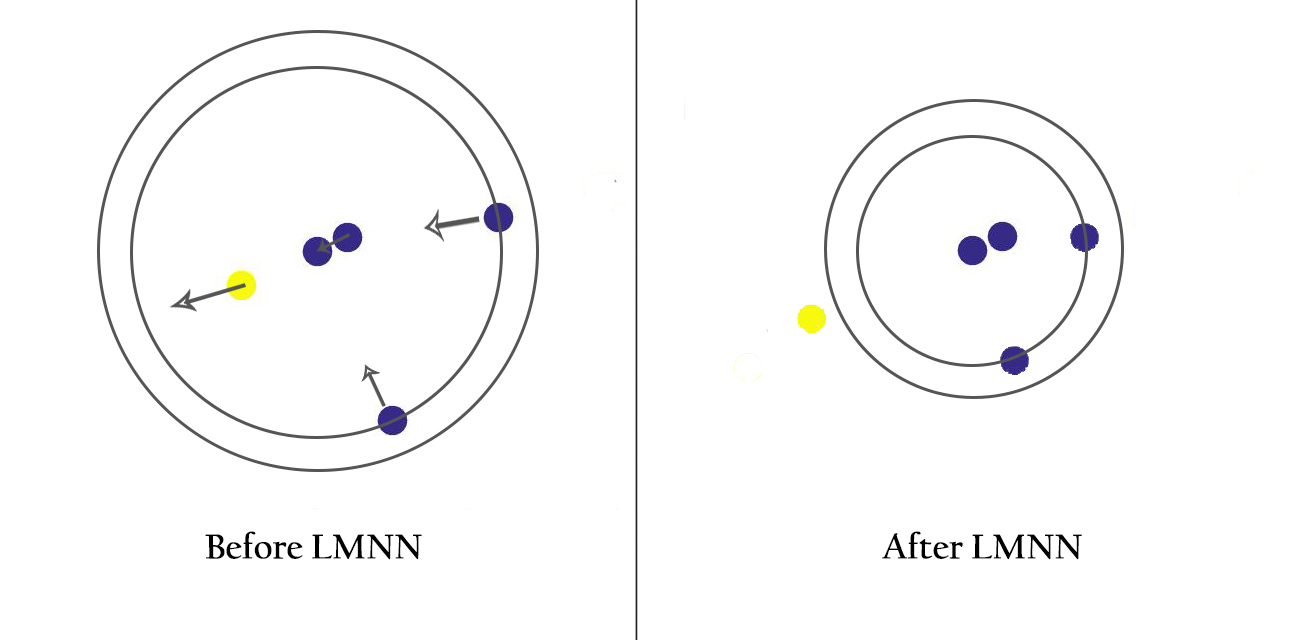
\includegraphics[width=1\textwidth]{lmnn}
    \caption{An example showing the motivation behind the use of the LMNN}
    \label{LMNN}
\end{figure}
The learning technique that is considered in this paper is the large margin nearest neighbors \cite{W09}. In the LMNN the ideal space would be one where each observation has the same class of its K nearest neighbors. This is done in the following way :
\begin{itemize}
\item Compute the pair wise Euclidean distance of the space.
\item Attract the K nearest neighbors corresponding to the same class(Shrink the distance between the observation and the k nearest corresponding to the same class).
\item Set a marge based on the farthest nearest neighbor from the same class.
\item Push all observations from different classes outside this marge(expand the distance between the observation and other samples that violate the margin.)
\end{itemize}
To better understand this idea, let us have a look at the following example in figure \ref{LMNN}. Consider a space of five samples that are divided in two classes. The blue class corresponds to samples played by a violin and the yellow class corresponds to samples played by a guitar. Let us focus on the effect of applying LMNN on the blue sample at the center. The settings of the LMNN will be tuned to a problem of three nearest neighbors classification. As showed in the first part of the figure \ref{LMNN}  that the three nearest neighbors to the blue sample in the middle are as follows : [Violin, Guitar, Violin]. The LMNN algorithm will thus aims to attract the two other samples that correspond to the violin class. To insure that the guitar will not be one of the nearest neighbors of that sample a margin will be set and the yellow sample should be pushed outside the margin. If the LMNN is applied with success the result will be similar to the second part of the figure \ref{LMNN}. The same process will be applied to each sample of the space.
\subsubsection{Learning a Mahalanobis distance}
To perform the process explained above, the LMNN uses a projection of the space by computing a Mahalanobis distance. A Mahalanobis distance is defined as follows  : $$D_\textbf{M}(\vec{x_i},\vec{x_j})=(\vec{x_i}-\vec{x_j})^T\textbf{M}(\vec{x_i}-\vec{x_j})$$
By considering M as  a positive semidefinite matrix M can be decomposed as follows : $$M=L^TL$$. Thus the Mahalanobis distance can be looked at as being a projection from an euclidean space to another euclidean space using the operator L : $$D_\textbf{L}(\vec{x_i},\vec{x_j})=||\textbf{L}(\vec{x_i}-\vec{x_j})||$$. By using this projection, the same process can be applied to obtain the ranking metrics (MAP and P@5).
\subsubsection{The Model}
 The model to solve this distance learning problem is based on three different optimization problems : \begin{enumerate}
\item Mahalanobis metric for clustering(MMC). \cite{X02}
\item Pseudometric Online Learning Algorithm(POLA) . \cite{S04}
\item Neighborhood Component Analysis(NCA). \cite{G05}
\end{enumerate}
The model formulates the parameter estimation as a convex optimization over the space of positive semidefinite matrices similar to the MMC. The margin by which the classifier is accurate for labeled examples will be maximized similar to POLA. And it is build to learn a Mahalanobis distance for optimization of K-NN classifier accuracy similar to the NCA. 
\subsubsection{The loss function}
The end result of applying LMNN would be to efficiently attract the k nearest neighbors and push impostors outside a certain margin. This formulations leads to a two termed loss function. The penalization is defined as follows : \begin{enumerate}\item Impose penalty on large distances between each sample and the k nearest neighbors with the same class label.
\item Impose penalty on small distances between each sample and samples corresponding to different classes.
\end{enumerate}
Before presenting the equations of the two terms of the loss function lets first give the notation that will be used. \par A target neighbor is one of the k nearest neighbors for each sample that correspond to the same class of that sample. The notation for such neighbor is the following : $j \rightsquigarrow i$ indicates that $\vec{x_j}$ is a target neighbor of $\vec{x_i}$. \\
An impostor is a neighbor that violates the marge set by the distance of each sample. This impostor will have a different label than the observation : $\vec{y_l}\neq \vec{y_i}$.\\
The equation will be presented in terms of the linear transformation L of the input space.\par 

Now that the terminology is presented, let us start by giving the equation of the first term of the loss function. This term is the one responsible of pulling the K-nearest neighbors corresponding to the same class as the observation and is given by :

 $$\epsilon_{pull}(L)=\Sigma_{j \rightsquigarrow i}||L(\vec{x_i}-\vec{x_j})||^2$$
 The first term of the loss function is thus being put on the sum of the distances between the observation and the k nearest neighbors corresponding to the same class in the projected space.\par
The second term of the loss function will push the impostors outside a defined margin. It is defined as follows : \par 
$\epsilon_{push}(L)=\sum\limits_{i, j \rightsquigarrow i}\sum\limits_{l}(1-y_{il})[1+||L(\vec{x_i}-\vec{x_j})||^2-||L(\vec{x_i}-\vec{x_l})||^2]_+$ \par 
A factor $y_{il}$ is introduced and it is equal to 1 if the observations i and l are from the same class and 0 otherwise. This factor will guarantee that this term will only affect the observations that are from different class than the observation i. In the equation, the margin that the observation should be pushed outside of it is defined as follows : $1+||L(\vec{x_i}-\vec{x_j})||^2$. From this margin, the distance between each observation and the one that correspond to different classes is subtracted. Only the positive value of the subtraction is taken to ensure that the penalization is being put on the observations that violates the margin. The sum of the distances is made on the entire space.\par 
Now that the two terms are defined we define the loss function as the pondered sum of those two factors. The equation is given as follows : 
$\epsilon(L)=(1-\mu)\epsilon_{pull(L)}+\mu \epsilon_{push}(L) $

Once the optimization problem is solved, The result will be the matrix L which will project the observations into a space that will better represent the data. Before applying the LMNN to the ground truth labeling problem, it will be applied to the true labeling problem to test its effect on the musical space for features extracted using the MFCC and the scattering.

\subsection{LMNN applied to the true labeling problem}
After preprocessing the data in the MFCC and the scattering space, the LMNN will be applied. At first the data will not be divided into a part for training and a part for testing. Rather the application of the LMNN will be on the hole data set and the results will be also on the hole data set.
\begin{table} [H]
\begin{center} 
\ 
 \setlength{\tabcolsep}{.16667em} 
\begin{tabular}{|l|l|l|} 
\hline
features & p@5 before LMNN & p@5 after LMNN \\ 
\hline 
16 class of instruments \\ 
\hline
mfcc & 86.89& 87.09  \\ 
scattering & 93.87 & 99.99  \\ 

\hline 
32 class of instruments with variation \\ 
\hline
mfcc & 85.12 & 86.16  \\ 
scattering & 90.94 & 99.92  \\ 
\hline 
498 class of playing techniques \\ 
\hline
mfcc &  45.19 & 46.38  \\ 
scattering & 57.98 & 88.08  \\ 
\hline
\end{tabular} 
\end{center} 
\caption{Comparison between the P@5 before and after LMNN for feature extracted using the MFCC and the scattering with T=250ms} 
\label{you} 
\end{table}

The first table shows the comparison between the P@5 before and after applying the LMNN. An improvement is noted for all the different type of classes for both features extracted using the MFCC and the scattering. The scattering continue to outperform the MFCC after the LMNN. For the two type instruments the scattering after the LMNN gives almost a perfect result. And for the last type of classes of playing techniques, the scattering after gives a remarkable improvement of 30.1\%.

  \begin{table} [H]
\begin{center} 
\ 
 \setlength{\tabcolsep}{.16667em} 
\begin{tabular}{|l|l|l|} 
\hline
features & MAP before LMNN & MAP after LMNN  \\ 
\hline 
16 class of instruments \\ 
\hline
mfcc         &     24.22& 24.73   \\ 
scattering   &30.73  & 60.07 \\ 

\hline 
32 class of instruments with variation \\ 
\hline
mfcc &22.29 & 25.27  \\ 
scattering &28.07& 56.88  \\ 
\hline 
498 class of playing techniques \\ 
\hline
mfcc &  8.78 & 9.61  \\ 
scattering &20.41& 44.42  \\ 
\hline
\end{tabular} 
\end{center} 
\caption{Comparison between the MAP before and after LMNN for feature extracted using the MFCC and the scattering with T=250ms} 
\label{you} 
\end{table}
Again for the MAP, The scattering continues to outperform the MFCC. with a big improvement after applying the LMNN. This shows that the scattering contains the necessary variability for the problem of music search query.\par
To further show the importance of the LMNN, two division of train test is made on the space and the results are shown in the following tables for the 32 class of instrument with variation:
\begin{table} [H]
\begin{center} 
\ 
 \setlength{\tabcolsep}{.16667em} 
\begin{tabular}{ | l | l | l | l | l |l|}
\hline
features & MAP before LMNN & MAP after LMNN  \\ 
\hline 
Division into 80\% for train and 20\% for test \\
\hline
mfcc & 23.24& 24.54  \\ 
scattering &31.00& 60.70    \\ 
\hline
Division into 50\% for train and 50\% for test \\
\hline
mfcc & 22.74& 24.02  \\ 
scattering & 30.70 & 62.98  \\ 
\hline
\end{tabular} 
\end{center} 
\caption{Results of the MAP for the division of the space into a part for train and a part for test} 
\label{you} 
\end{table} 
The first table shows that for both the mfcc and the scattering an improvement was noted even with a split of 50/50 between train and test. However for the scattering  the improvement was greater and it provided the same improvement without the division into train test.

\begin{table} [H]
\begin{center} 
\ 
 \setlength{\tabcolsep}{.16667em} 
\begin{tabular}{ | l | l | l | l | l |l|}
\hline
features & P@5 before LMNN & P@5 after LMNN  \\ 
\hline 
Division into 80\% for train and 20\% for test \\
\hline
mfcc & 73.90& 75.14  \\ 
scattering &83.05& 98.44    \\ 
\hline
Division into 50\% for train and 50\% for test \\
\hline
mfcc & 81.17& 81.86  \\ 
scattering & 90.02 & 99.31  \\ 
\hline
\end{tabular} 
\end{center} 
\caption{Results of the P@5 for the division of the space into a part for train and a part for test} 
\label{you} 
\end{table} 
The same can be noted for the P@5. The division was made on the entire space by taking 80\% of each class for train and 20\% for test(50\% for train and 50\% for test from each class). \par
Now that the effect of LMNN have been proven to be very effective on the scattering while it provides slight improvement for the MFCC, one last test should be made. This test is to prove that the effectiveness of the LMNN on the scattering is not due to the space volume rather than the variability this space contains. \\
The MFCC was extended in the following way :
\begin{itemize}
\item add the delta coefficients (a total of 12 coefficients) 
\item add the delta delta coefficients (a total of 12 coefficients)
\item Multiply the pair wise coefficients, the total will 666 coefficients $$((36*35)/2)+36=666$$
\end{itemize}
Then the same number of coefficients is taken from the scattering. The results are given in the following table : 
\begin{table} [H]
\begin{center} 
\ 
 \setlength{\tabcolsep}{.16667em} 
\begin{tabular}{ | l | l | l | l | l | l |}
\hline
features & MAP before LMNN& map after LMNN & p@5 before LMNN & p@5 after LMNN \\ 
\hline 
mfcc & 10.38 & 13.35 & 58.01 & 77.80 \\ 
scattering & 28.43 & 51.35 & 92.85 & 99.85  \\ 
\hline
\end{tabular} 
\end{center} 
\caption{Table showing the comparison between the scattering and the MFCC with the same number of features (666) before and after applying the LMNN} 
\label{you} 
\end{table} 
The results shown in the table above were anticipated. The scattering transform outperformed the MFCC after applying the LMNN even when the space of MFCC features was expended. The MFCC precision degraded with the additional features. The LMNN could not rise the precision of the MFCC even with a high space of features.\par 
Now that the LMNN has proven to be efficient for the musical search query problem based on the physical labeling of the observation, it is time to see its effect on the ground truth problem.
\subsection{LMNN applied to the ground truth problem}
To apply the LMNN to a series of multiple labeling opinion some alternation should be made. It should be noted that this problem was not addressed before. Many methods were proposed and tested to take advantage of the LMNN to make it adaptable to the problem : 
\begin{enumerate}
\item \textbf{Summing the distances} \par 
The first method that was proposed is to sum over the distances. Two ways of summing the distances was used :\par The first one is to sum over the matrices L of projection obtained by the LMNN. To better understand the difference between this approach and summing directly the distances let us see the equations below : \\
Summing the projection matrices L can be written as :
$$L=\sum_{k=1}^{nobs}L_k$$
Thus the new distances will be :
 $$(\vec{x_i}-\vec{x_j})^T\sum_{k=1}^{nobs}L_k^T\sum_{k=1}^{nobs}L_k(\vec{x_i}-\vec{x_j})$$
  $$=(\vec{x_i}-\vec{x_j})^T\sum_{k=1,w=1}^{nobs}L_k^TL_w(\vec{x_i}-\vec{x_j})$$
  $$=(\vec{x_i}-\vec{x_j})^T(\sum_{k=1,w=1,k=w}^{nobs}L_k^TL_w+\sum_{k=1,w=1,k\neq w}^{nobs}L_k^TL_w)(\vec{x_i}-\vec{x_j})$$
   $$=(\vec{x_i}-\vec{x_j})^T\sum_{k=1,w=1,k=w}^{nobs}L_k^TL_w(\vec{x_i}-\vec{x_j})+(\vec{x_i}-\vec{x_j})^T\sum_{k=1,w=1,k\neq w}^{nobs}L_k^TL_w(\vec{x_i}-\vec{x_j})$$
  $$\sum_{k=1}^{nobs}d_{M_k}(\vec{x_i}-\vec{x_j})+\sum_{k=1,w=1,k\neq w}^{nobs}(L_k\vec{x_i}-L_k\vec{x_j})^T(L_w\vec{x_i}-L_w\vec{x_j})\ \ eq.1$$
 The first part of eq.1 is the same as summing the distances directly, the second part however do not have a physical explanation. A sum over the distance is better understood. However a comparison is provided for further study since it achieved good results.
 
 \begin{table}[H]
\begin{center} 
\ 
 \setlength{\tabcolsep}{.16667em} 
\begin{tabular}{ | l | l | l | l | l | l | l |} 
\hline
features & Sum & MAP & MAP after LMNN & p@5 & p@5 after LMNN  \\ 
\hline 
mfcc & Sum over L& 50.74 &55.02 & 55.66 & 60.99 \\ 
mfcc & Sum over distances & 50.74 & 54.24 & 55.66 & 60.04  \\ 
scattering& Sum over L & 40.17 & 49.63 & 44.01 & 61.85  \\ 
scattering & Sum over distances & 40.17 & 51.46 & 44.01 & 65.57  \\
\hline
\end{tabular} 
\end{center} 
\caption{Results of summing the distances and summing the projection matrix L} 
\label{you} 
\end{table}
 
 
 
 
 
Lets look at all the different cases that might be encountered to better understand the improvement provided by the sum over the distances. In the following study, the focus is only on two different labeling opinions from the 32. The figure \ref{Lmnnsum} show an example of applying LMNN on two different labeling opinion for the same samples with three nearest neighbors considered. The pairwise distance matrix before applying the LMNN is given by :

\[
\begin{bmatrix}
    1            & d_{12} & d_{13}  & d_{14}  & d_{15} \\
    d_{21}       & 1      & d_{23}  & d_{24}  & d_{25} \\
    d_{31}       & d_{32} & 1       & d_{34}  & d_{35} \\
    d_{41}       & d_{42} & d_{43}  & 1       & d_{45} \\
    d_{51}       & d_{52} & d_{53}  & d_{54}  & 1
\end{bmatrix}
\]

After applying the LMNN with sum over distances Four different cases can be presented :
\begin{figure}[t!]
  
  \centering
	    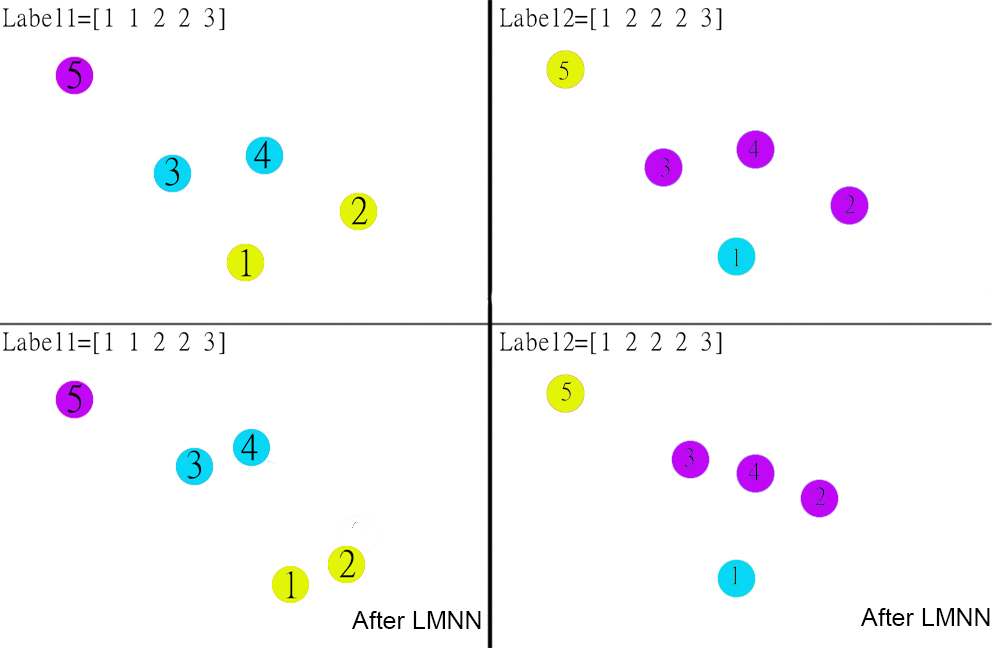
\includegraphics[width=1\textwidth]{lmnnex1}
    \caption{LMNN applied on two different labeling opinion}
    \label{Lmnnsum}
\end{figure}

\begin{enumerate}
\item The two labeling opinion agrees on the similarity.\\
The application of LMNN will conduct to a smaller distance if the labels are similar. If the observations are target neighbors both distances will be smaller in the new space for both labeling provided by the two different users. Observation 3 and 4 in figure 1 illustrate that idea. In this case the two distances $D_{M_1}$ and $D_{M_2}$ will be smaller than the original distance in the space before the application of LMNN. Let us now go back to update our new pair wise distance matrix: 
$$D_{M_1}34<d_{34}\  and \  D_{M_2}34<d_{34} $$ the sum of those two terms is thus : $$D_{M_1}34+D_{M_2}34<2d_{34}$$.
\item The two labeling opinion agrees on the non similarity.\\
The same analogy can be made for the case were both opinion agree that the two observation belongs to different classes. If we take for example the observations 1 and 3 we will have at the end  $$D_{M_1}34+D_{M_2}34>2d_{34}$$.
\item The two labeling opinion dos not agrees on the similarity.\\
If the two labeling opinion disagree on the similarity between two observation, in one space we will have smaller distance while in the second we will have bigger distance. For example if we look at samples  2 and 4 in figure 1, we can see that in the new spaces distance between those two observations is bigger for the new space with LMNN based on labeling opinion 1, and bigger in the space with LMNN based on labeling opinion 2. we will thus have : $$D_{M_1}24>d_{24} \ and \ D_{M_2}24<d_{24}$$. Let us introduce two factors $\alpha>1$ and $\beta<1$ this implies : $$D_{M_1}24=\alpha d_{24}\ and \ D_{M_2}24=\beta d_{24}$$
$$D_{sum}24=\alpha d_{24}+\beta d_{24}$$. 
\item An observation is not affected in both spaces by LMNN.\\
If the distance between two observations that are not target neighbors for the LMNN is bigger than a certain margin the distance will not be affected directly. This distance will slightly change because the observation themselves have been displaced in their own small margin. We can thus make the assumption that the variation in distance in the new space is negligible and the for example the distance between observation 1 and 5 will be $$D_{sum}15=2d_{15}$$
\end{enumerate}
Now that we have formulated all the factors we can construct our new matrix based on the sum of the projection matrix L. To simplify the notation we will take on factor to represent the different factors in case 3, for example let $2A=\alpha+\beta$.
\[
\begin{bmatrix}
1            & 2Ad_{12} & >2d_{13}  & >2d_{14} & 2d_{15} \\
2Ad_{21}     & 1        & 2Cd_{23}  & 2Bd_{24} & 2d_{25} \\
>2d_{31}     & 2Cd_{32} & 1         & <2d_{34} & 2d_{35} \\
>2d_{41}     & 2Bd_{42} & <2d_{43}  & 1        & 2d_{45} \\
2d_{51}      & 2d_{52}  & 4d_{53}   & 2d_{54}  & 1
\end{bmatrix}
\]
Let us now examine two cases, one were we have an agreement and one were we have a disagreement :
\begin{enumerate}
\item Case were we have agreement between different opinions.\\
It should be noted again that we are searching to compare distances and not the exact value of the distances. So let us take two distances were in the first both users agree that two samples belongs to the same class and in the other they agree that they don't.  for example we can take $d_{13} \ and \ d_{34}$. In the space before the application of LMNN we had : $d_{13}-d_{34}$ in the new space we will have a difference between a value that is twice bigger than the first distance and a value that is twice smaller than the second distance. So we have been able to have a space that make the difference in distances bigger if we have two exact opinions on labeling. And for both labeling opinions the error will be minimized.
\item Case were we have disagreement between opinions.
Let us take again distance $d_13$ but this time let us compare it with $d_21$. Let us take F as a value that is bigger than 1 to represent the factor by which in the new space the distance between samples 1 and 3 is bigger. we will thus have in the new space $2Fd_{13}-2Ad_{d21}$. We now that the first distance is going to be bigger than the original distance between samples 1 and 2. On the other hand the distance between 1 and 2 in the new space will depend on the original distance between 1 and 2. So if the distance in the new space is smaller than in the original space, labeling based on first user will have smaller error than labeling based on second user. But since the first factor is well optimized we will have optimization in both case. \\
This idea that the "winner" between the two opinion is based on the representation in the original space is very important. And it will be essential in a case were we have more than two opinions, since the probability that two samples will be considered similar by the users is related to the physical aspect of the sound. 
 \end{enumerate}
 \item \textbf{Pondering the sum over distances} \par 
In this case, the sum has been preponderated based on a factor of success of each labeling opinion relatively to the other labeling opinions. The success is based on a precision factor obtained by applying the normalized mutual information. The distances will thus be multiplied each one by the precision of the labeling opinion over the entire labeling opinion space. The results are as follows :
\begin{table} [H]
\begin{center} 
\ 
 \setlength{\tabcolsep}{.16667em} 
\begin{tabular}{ | l | l | l | l | l | l |}
\hline
features & MAP & MAP after LMNN & P@5 & p@5 after LMNN  \\ 
\hline 
mfcc & 50.74& 54.35 & 55.66 & 60.51  \\ 
scattering & 40.17 & 52.61 & 44.01 & 66.89  \\ 
\hline
\end{tabular} 
\end{center} 
\caption{Results of pondering the sum} 
\label{you} 
\end{table} 
 
 Pondering the distance provides inconsistent results. For the MFCC the effect is minimal whether for the scattering it provides improvement of around 1\%.
 
\item \textbf{Normalizing the distance}\par 
In this method, the distances has been normalized before performing the sum. This is to reduce the effect of big distances provided by one user over small distances provided by the rest for the same two observations. The results are presented in the following table :
\begin{table} [H]
\begin{center} 
\ 
 \setlength{\tabcolsep}{.16667em} 
\begin{tabular}{ | l | l | l | l | l | l | l |}
\hline
features & metrics & MAP & MAP after LMNN & P@5 & P@5 after LMNN  \\ 
\hline 
mfcc & normalized distance sum & 50.74 & 54.31 & 55.66 & 60.29  \\ 
mfcc & normalized pondered distance sum &50.74 & 54.39 & 55.66 & 60.09  \\ 
scattering & normalized distance sum & 40.17 & 54.03 & 44.01 & 67.33  \\ 
scattering & normalized pondered distance sum  & 40.17 & 54.30 & 44.01 & 67.63 \\ 
\hline
\end{tabular} 
\end{center} 
\caption{Results of normalizing the distances} 
\label{you} 
\end{table}  
 Normalizing before effecting the sum proved to be beneficial for the scattering and not for the MFCC. This is due to the high conventionality of the scattering that might have an affect over the distances. This effect will be reduced by applying a normalization over the distances.
 \item \textbf{Class Matching} \par 
 The last method that was tested is to apply a class matching over the space of different observation. This is done using the NMI(normalized mutual information) technique. After matching the space of opinions, all the classes will be well aligned. Now using a majority vote over the space of observations, only one label will obtained. The LMNN will be thus trained only once on the obtained labeling. This will induce a shorter amount of training time and a faster algorithm. The results are given in the following table : 
 \begin{table}[H] 
\begin{center} 
\ 
 \setlength{\tabcolsep}{.16667em} 
\begin{tabular}{ | l | l | l | l | l | l |}
features & map & mapafter & pat5 & pat5after\\ 
\hline 
mfcc & 50.74 & 55.34 & 55.66 & 61.77 \\ 
scattering & 40.17 & 49.41 & 44.01 & 60.75  \\  
\end{tabular} 
\end{center} 
\caption{metrics: lmnnclassmatching, type: instrument16GT} 
\label{you} 
\end{table}  
The class matching proved to be beneficial for the MFCC over the sum of distances. For the scattering summing the distances is better but with dramatically more computation time : For the class matching 21.01 seconds and for the sum of distances 2316.59 seconds.  
\end{enumerate}

\section{Conclusion}
This paper provided a study of two problems of music search query. The first one based on the physical aspect of the sound. The results obtained for this part and the preprocessing technique for the scattering are novel work. The precision obtained on the search query for musical purposes proved that the standard deviation of the scattering should be studied in order to achieve state of the art results. This technique of preprocessing should be tested for different problems in the domain of audio and images.
In the second part, the problem of studying multiple user opinion in order to find a space that respects all the opinions was addressed. This novelty work has put some new foundation for solving the problem.
\newpage
\begin{thebibliography}{2}
\bibitem{B00} 
Beth Logan
\textit{Mel Frequency Cepstral Coefficients for Music Modeling}. 
2000

\bibitem{AM11} 
J. Andén and S. Mallat. 
\textit{Multiscale scattering for audio classification.}. 
ISMIR 2011

\bibitem{A14} 
J. Andén 
\textit{Time and frequency scattering for audio classification}. 
January 7, 2014

\bibitem{H95}
Hermann Ludwig Ferdinand von Helmholtz
\textit{On the sensations of tone as a physiological basis}.
1895

\bibitem{M10}
Stephan Mallat 
\textit{Recursive interferometric Representations}  18th European Signal Processing Conference 2010
\bibitem{P03}
Perfecto Herrera-Boyer and al.
\textit{Automatic Classification of Musical Instrument Sounds}.
Journal of New Music Research 2003


\bibitem{SOL}
Yan Maresz and al.
\textit{Ircam solo instruments UltimateSoundBank reference guide}

\bibitem{W09}
K. Q. Weinberger, L. K. Saul. 
\textit{Distance Metric Learning for Large Margin Nearest Neighbor Classification}.
Journal of Machine Learning Research (JMLR) 2009

\bibitem{X02}
P. Xing, A. Y. Ng, M. I. Jordan, and S. Russell 
\textit{Distance metric learning, with application to
clustering with side-information}.
 Cambridge, MA, 2002.
 \bibitem{S04}
 Shalev-Shwartz, Y. Singer, and A. Y. Ng.
 \textit{Online and batch learning of pseudo-metrics}
 Banff, Canada, 2004.
 \bibitem{G05}
 Goldberger, S. Roweis, G. Hinton, and R. Salakhutdinov.
 \textit{Neighbourhood components analysis}
 Cambridge, MA, 2005
\end{thebibliography}
\end{document}